
\subsection{Graphics processing units}

\begin{frame}[t]
\frametitle{Introduction}
\pause
\begin{columns}[T]
\begin{column}{0.4\textwidth}
\begin{itemize}
    \item <2-> Highly multi-threaded processor
        \begin{itemize}
            \item NVIDIA Tesla K20 accelerator: 2496 cores
        \end{itemize}
    \item <3-> Spectacular performance for
        \emph{compute-intensive, data-parallel} operations
    \item <4-> Not suited for general-purpose computation
    \item <5-> Requires careful redesign of algorithms,
        substantial code changes, and tuning efforts
\end{itemize}
\end{column}
\begin{column}{0.6\textwidth}
\visible<2-> {
    \vspace{2cm}
    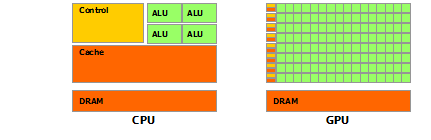
\includegraphics[width=180px]
    {img/device-comparison.png}
}
\end{column}
\end{columns}
\end{frame}

\begin{frame}
\frametitle{Programming GPUs}
\pause
Scientific applications use GPUs at various levels:
\begin{itemize}
    \item Low-level
        \begin{itemize}
            \item CUDA
            \item OpenCL
        \end{itemize}
    \item High-level
        \begin{itemize}[<+->]
            \item OpenACC compiler directives
            \item Drop-in support for scientific libraries such as Intel MKL, BLAS
        \end{itemize}
    \item Transparent
        \begin{itemize}[<+->]
            \item MATLAB: over 200 functions
            \item Software packages: Abaqus, ANSYS (Mechanical/Fluent)
        \end{itemize}
\end{itemize}
\end{frame}

\begin{frame}
\frametitle{CUDA programming model}
\pause
\begin{columns}
\begin{column}{0.5\textwidth}
\textbf{Kernels}
\begin{itemize}[<+->]
    \item Special pieces of code that execute on the GPU
    \item In Fortran: subroutines; in C: functions
    \item Executed concurrently by several GPU threads
\end{itemize}
\textbf{Threads}
\begin{itemize}[<+->]
    \item Threads organized into a grid of blocks
    \item Kernels launched with specified grid size
        (number of blocks) and block size (threads per block)
    \item Grid and blocks can be 2-D or 3-D for convenience
\end{itemize}
\end{column}
\begin{column}{0.5\textwidth}
    \only<5-6>{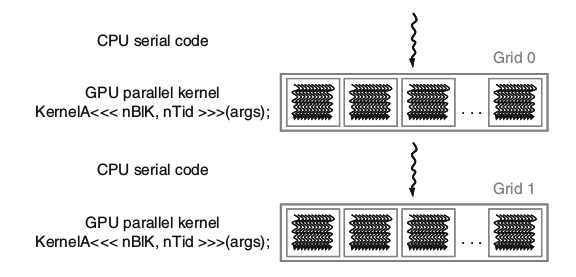
\includegraphics[width=150px]{img/program-structure.png}}
    \only<7>{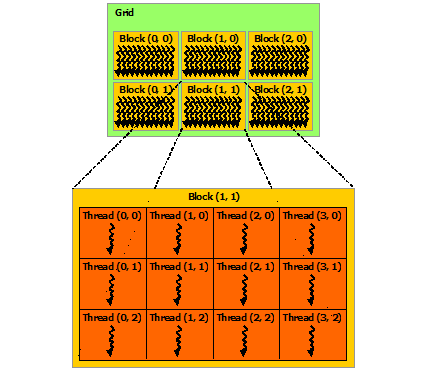
\includegraphics[width=150px]{img/grid-of-thread-blocks.png}}
\end{column}
\end{columns}
\end{frame}

\begin{frame}
\frametitle{GPU architecture and memory model}
\pause
\begin{columns}
\begin{column}{0.5\textwidth}
\begin{itemize}[<+->]
    \item GPU viewed as a collection of \emph{streaming microprocessors} (SMs)
    \item When kernel is launched, each block gets assigned to an SM
    \item Threads within a block execute concurrently
    \item SM may execute several blocks concurrently
\end{itemize}
\end{column}
\begin{column}{0.5\textwidth}
    \visible<3->{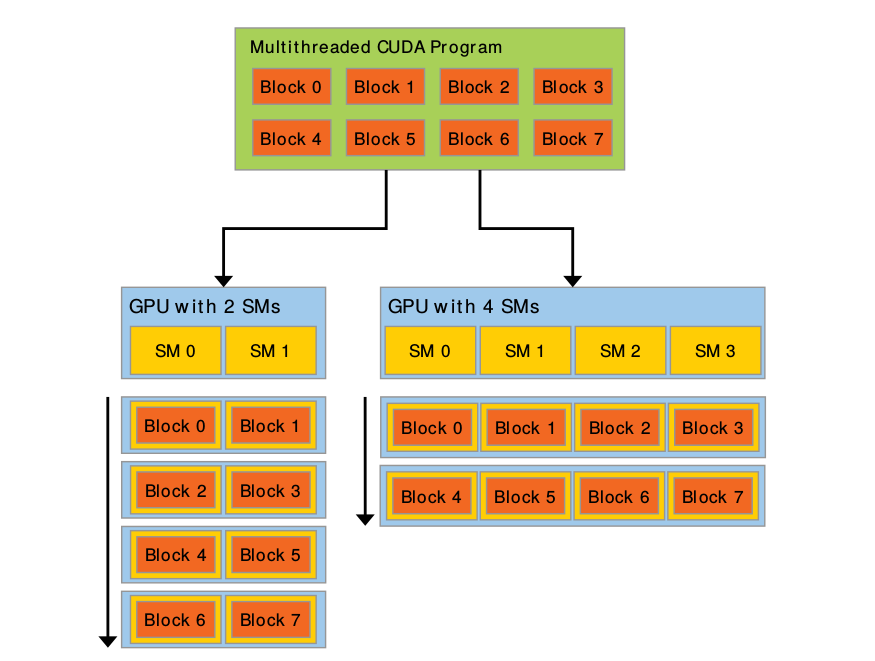
\includegraphics[width=150px]{img/gpu-scaling.png}}
\end{column}
\end{columns}
\end{frame}

\begin{frame}
\frametitle{GPU architecture and memory model}
\pause
\begin{columns}
\begin{column}{0.5\textwidth}
\begin{itemize}
    \item Global memory{
        \begin{itemize}
            \item large but slow (~5 GB for Tesla K20)
            \item all threads can access
            \item persists between kernel launches
        \end{itemize}}
    \item Shared memory{
        \begin{itemize}
            \item small but fast (~48 KiB per SM)
            \item local to threads within a block
            \item explicitly managed cache
        \end{itemize}}
    \item Registers{
        \begin{itemize}
            \item limited (65536 per SM)
            \item local to individual threads
            \item fastest
        \end{itemize}}
\end{itemize}
\end{column}
\begin{column}{0.5\textwidth}
    \visible<2->{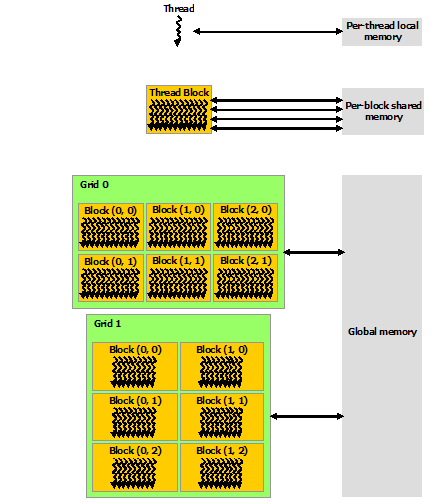
\includegraphics[width=150px]{img/memory-hierarchy.png}}
\end{column}
\end{columns}
\end{frame}

